\documentclass[11pt,a4paper]{scrartcl}
\usepackage[utf8]{inputenc}
\usepackage{float}
\usepackage{amsmath}
\usepackage{amsfonts}
\usepackage{amssymb}
\usepackage{graphicx}
\usepackage{color}
\usepackage[english, russian]{babel}


\begin{document}
\begin{flushright}
	Егерев Артем \\
	Домашнее задание №18 \\
\end{flushright}
\textbf{\Large Задача 1}
\medskip\hrule\medskip
\textsl{Докажите, что функцию  $ x \oplus y \oplus z $  можно вычислить схемой, использую лишь одно отрицание (и много конъюнкций и дизъюнкций).}
\\ \\
\fbox{\textit{Решение: }} \\ \\

\noindent Рассмотрим все варианты, когда функция дает нам положительный результат $ \rightarrow $ сумма равна 1 или 3 по модулю 2 $ \Rightarrow $ 2  варианта: одна из переменных равна 1, остальные 0 или все равны 1. \\
Первое есть $ (x \land y \land z) $ \\
Второе есть $ \neg((x \land y) \lor (x \land z) \lor (y \land z)) \land  (x \lor y \lor z)$ \\ 
В виде схемы это будет выглядеть следующим образом:
\begin{center}
	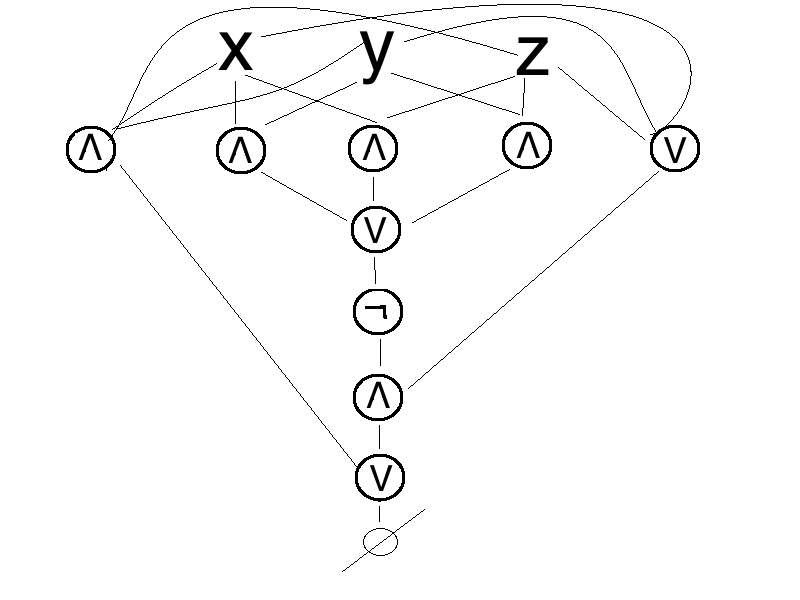
\includegraphics[height = 100mm]{1.png}
\end{center}
\newpage

\textbf{\Large Задача 2}
\medskip\hrule\medskip
\textsl{Функция $ f(x_1, x_2, x_3, x_4) $  истинна на последних 9 наборах значений переменный (в стандатрном порядке) и только на них. Постройте схему, вычисляющая $ f $, использующую только диъюнкцию и конъюнкцию длины не более  чем 15.}
\\ \\
\fbox{\textit{Решение: }} \\ \\
Выпишем в таблицу значения, на которых функция равна 1:
\begin{center}
	\begin{tabular}{|c|c|c|c|}
		\hline
		 $ x_1 $ &  $ x_2 $ & $ x_3 $ & $ x_4 $ \\
		\hline 
		0 & 1 & 1 & 1 \\ 
		\hline
		1 & 0 & 0 & 0 \\ 
		\hline
		1 & 0 & 0 & 1 \\ 
		\hline
		1 & 0 & 1 & 0 \\ 
		\hline
		1 & 0 & 1 & 1 \\ 
		\hline
		1 & 1 & 0 & 0 \\ 
		\hline
		1 & 1 & 0 & 1 \\ 
		\hline
		1 & 1 & 1 & 0 \\ 
		\hline
		1 & 1 & 1 & 1 \\ 
		\hline
	\end{tabular}
\end{center}
$ \Rightarrow f(x) \Longleftrightarrow x_1 \lor (x_2 \land x_3 \land x_4)$ : 
\begin{center}
	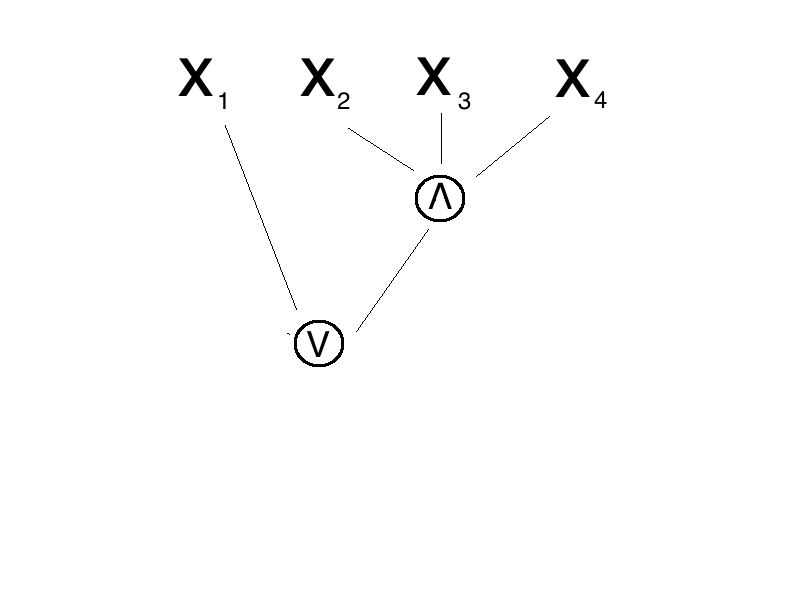
\includegraphics[height = 100mm]{2.png}
\end{center}
Размер схемы - 11 < 15.
\newpage


\newpage
 

\textbf{\Large Задача 3}
\medskip\hrule\medskip 
\textsl{Постройте схему полиномиального размера, проверяющую, что во входное слово входит подслово 101. Можно считать, что длина входного слова не меньше, чем 3} \\ \\
\fbox{\textit{Решение: }} \\ \\
Пусть  $ n $ - размер входного слова.
Тогда наша схема запишется в строку:
\begin{align*}

	x_1, x_2 ... x_n; \\
	\textit{ }\overline{x_2}, \overline{x_3} ... \overline{x_{n - 1}}\textit{ }; \\
	(x_1 \land \overline{x_2} \land x_3), (x_2 \land \overline{x_3} \land x_4), ... (x_{n - 2} \land \overline{x_{n - 1}} \land x_{n}); \\
	(x_1 \land \overline{x_2} \land x_3) \lor (x_2 \land \overline{x_3} \land x_4) ... (x_{n - 2} \land \overline{x_{n - 1}} \land x_{n});
\end{align*}
Оценим теперь рамер этой схемы. На каждом из 4 этапов мы вычисляем не более $ n $ элементов $ \Rightarrow $  как следствие, суммарно нам потребуется $ O(n) $ элементов.
\\ \\ \\

\textbf{\Large Задача 4}
\medskip\hrule\medskip 
\textit{Посройте схему полиномиального размера, умнощающее двоичное число на 3.} \\ \\
\fbox{\textit{Решение: }} \\ \\ 
Для удобства определим сразу функции, которыми мы будем пользоваться в дальнейшем : \\
\begin{gather*}
	XOR(x, y) \Leftrightarrow x \oplus y:\\  x, y; \quad \overline{x}, \overline{y}; \quad (\overline{x} \land y), (x \land \overline{y}); \quad (\overline{x} \land y) \lor (x \land \overline{y}) \\ \\
	MAJ(x, y, z): \\
	x, y, z;\quad \overline{x}, \overline{y}, \overline{z}; \quad (x \land y), (x \land z), (y \land z); \quad (x \land y) \lor (x \land z) \lor (y \land z)	
\end{gather*}
Умножение на 3 есть сумма 3 чисел, равных данному, поэтому для определения схемы нам достаточно определить сложение двух двоичных чисел: пусть $ n $ - длина большего числа, тогда первое число в сумме представимо в виде : $\overline{ a_n a_{n - 1}...a_1 a_0 }$, второе: $\overline{ b_n b_{n - 1}...b_1 b_0 }$. Будем записывать в $ c_i $ дополнительную единицу, которая получается при сложение (по аналогии с обычным сложением). Обозначим результат сложения за: $\overline{ d_{n + 1} d_{n}...d_1 d_0 }$. $ c_0 = 0 $ соответственно. Тогда, для каждого $ i $ от $ 0 \text{ до } n + 1$: $ d_i = a_i \oplus b_i \oplus c_i$; $ c_{i + 1} = MAJ(a_i, b_i, c_i) $ (исходя из правил сложения). Таким образом, мы можем однозначно определить нашу схему. \\ \\
Оценим теперь размер этой схемы. Нам нужно посчитать сумму 2 раза. Для каждого разряда нам нужно не более 2-х раз применить подсхему для вычисления $ \oplus $ и не более 1-ого раза подсхему для вычисления $ MAJ_3 $. Все схемы имеют постоянный размер, отсюда нам нужно всего $ O(n) $ элементов.
\\ \\ \\

















\textbf{\Large Задача 5}
\medskip\hrule\medskip 
\textit{Постойте схему полиномиального размера, проверяющую, будет ли $ n $ - битное двоичное число делиться на 3.} \\ \\
\fbox{\textit{Решение: }} \\ \\ 
Двоичное число представимо в виде: $ a = \overline{a_n a_{n - 1} ... a_1 a_0}  = a_n 2^n + a_{n - 1}2^{n - 1} ... + a_1 2^1 + a_0$. Посмотрим какой остаток дает нам каждое слагаемое при деление на 3:\\
\[
	\begin{cases}
	a_k 2^{2i} \equiv a_k 4^i \equiv a_k \textit{ по модулю 3} & \textit{// при четном $ k $}\\
	a_k 2^{2i + 1} \equiv a_k 4^i \cdot 2 \equiv -a_k \textit{ по модулю 3} & \textit{// при нечетном $ k $}\\
	\end{cases}
\]
$ \Rightarrow a \equiv a_0 - a_1 + a_2 ... $ по модулю 3.\\
Найдем остаток $ a $ при деление на 3. Для этого мы введем 2 бита $ u_1 $ и $ u_2 $, 
которые будут равны $ \overline{u_1 u_2} $ =  00, 01, 10 и будут символизировать остатки 0, 1, 2 соответственно. \\ \\
Изначально $ \overline{u_1 u_2} = 00$. Далее мы будем идти по каждой цифре и в зависимости от индекса $ k $  и значения $ a_k $  менять значения $ u_1, u_2 $ на:
\[
\begin{cases}
	k - \textit{четное} \begin{cases}
							a_k = 0 & (0, 1, 2) \rightarrow (0, 1, 2) \\
							a_k = 1 & (0, 1, 2) \rightarrow (1, 2, 0) \\
						\end{cases} \\
	k - \textit{нечетное} \begin{cases}
							a_k = 0 & (0, 1, 2) \rightarrow (0, 1, 2) \\
							a_k = 1 & (0, 1, 2) \rightarrow (2, 0, 1) \\
	\end{cases}
\end{cases}
\] 
Таким образом, если в конце  мы получаем $ \overline{u_1 u_2} = 00 \Rightarrow a \textit{ }\vdots \textit{ }3$ \\  
Теперь по-подробнее как мы производим следующие преобразования (новые $ u_1, u_2$  относительно старых $ u'_1, u'_2$):
\begin{gather*}
	(0, 1, 2) \rightarrow (0, 1, 2): \\
	u_2 = u'_2 \\
	u_1 = u'_1 \\
	(0, 1, 2) \rightarrow (1, 2, 0): \\	
	u_2 = \overline{u'_1} \land \overline{u'_2} \\
	u_1 = u'_2 \\
	(0, 1, 2) \rightarrow (2, 0, 1): \\	
	u_2 = u'_1 \land \overline{u'_2} \\
	u_1 =  \overline{u'_1} \land \overline{u'_2} \\
\end{gather*}
Запихнув в один блок обработку 2-х последовательных  цифр числа (тем самым сразу обработав одно четное и одно нечетное $ k $) мы получаем в этом блоке константное количество действий. Оценим теперь размер этой схемы. Нам нужно зайти в блок не более, чем $ \lceil\frac12 n \rceil$ раз. Каждый блок это константа. Отсюда нам нужно всего $ O(n) $ элементов.
\newpage


































\end{document}
